
\documentclass{article} 
\usepackage{graphicx} 
\usepackage{amsmath}

% Increase margins (manually) 
  % Sides (odd- and even-numbered pages)
    \addtolength{\oddsidemargin}{-0.875in}
    \addtolength{\evensidemargin}{-0.875in}
    \addtolength{\textwidth}{1.75in}
  % Top/bottom
    \addtolength{\topmargin}{-0.875in}
    \addtolength{\textheight}{1.75in}

\begin{document}


\title{ASTR 565} \author{Laurel Farris}

\maketitle

\section{Problem 1.1: Variation of Luminosity with $\epsilon$}

The amount of energy generated by nuclear fusion in a star per second
per unit mass is characterized by $\epsilon$ [erg
g\textsuperscript{-1} s\textsuperscript{-1}]. This can be expressed 
as 
%\begin{equation}
  $\epsilon$ = $\frac{dL}{dm}$ 
%\end{equation}
  or 
%\begin{equation}
  $dL = \epsilon dm$,                       
%\end{equation}
where $L$ is luminosity and $m$ is mass. 
If $\epsilon$ = 0, then $dL$ = 0, implying a constant $L$. 
Figure \ref{fig1} shows a plot of both $\epsilon$ and $L$ as functions
 of mass, normalized to a fraction of their maximum values. They 
illustrate
that $L$ only changes when $\epsilon$ has a value
greater than zero. When $\epsilon$ falls back to zero, $L$ is again
constant at its maximum value. 
\begin{figure}[h] \centering
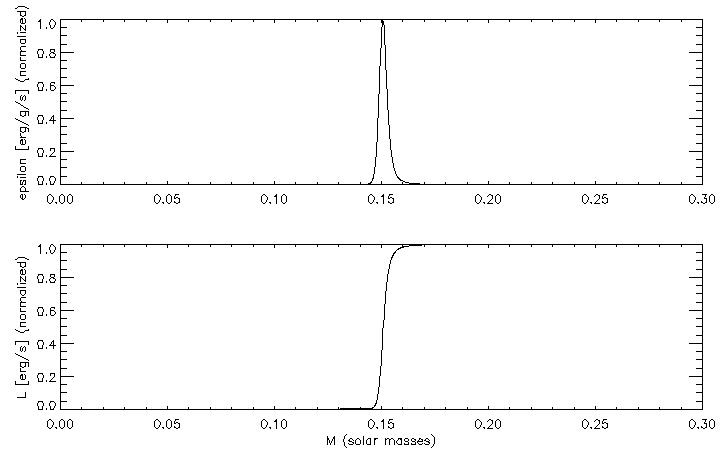
\includegraphics[width=5.0in]{../q01/fig1.jpg} \caption{Variation of
$\epsilon$ (top plot) and L (bottom plot) with mass.} \label{fig1}
\end{figure}

Given the value on the x-axis at which these changes occure, 
this would suggest that nuclear
reactions occur in a region containing about 15\% of the star's
total mass. 

The values for these figures were obtained from the results of a model 
run using Modules for Experiments in Stellar 
Astrophysics (MESA). 

\newpage

%--------------------------------------------------------------------%

\section{Computer Problem 1.1: Effects of nuclear fusion reactions on
the evolution of a star}

\subsection{Procedure} Two solar-mass stellar models were run using
MESA. The first
(`Model 1' henceforth) was run with the nuclear reactions rates turned
off and was set to stop after reaching an age of 10 billion years. The
second (`Model 2') was run with the nuclear reactions turned back on
and set to stop just after the onset of hydrogen fusion, when the hydrogen
 abundance dropped below 0.7.
	
\subsection{Results} The stellar model that included hydrogen fusion
stopped when the star reached an age of about 1.5 billion years.
Figure \ref{fig2} shows an H-R diagram of both stars.  The model with
no nuclear burning reached a maximum temperature of about 21000 K
while the model that included nuclear burning only reached a 
temperature of about 5600
K. 

\begin{figure}[h] \centering 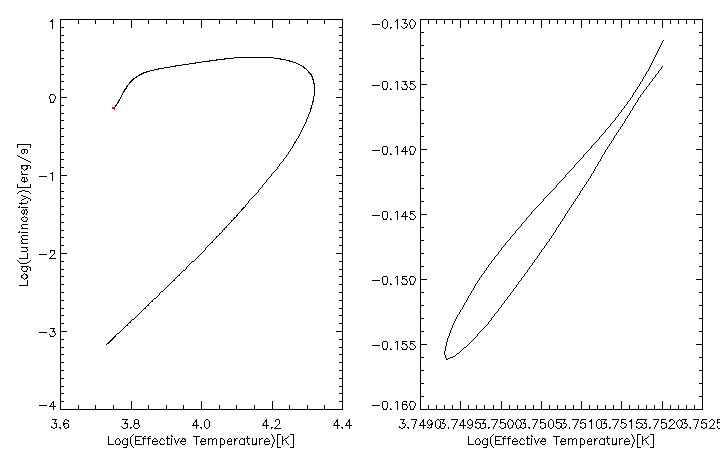
\includegraphics[width=5.0in]{fig2.png}
\caption{These H-R diagrams show the evolutionary tracks of both
models. Model 1 is on the left, aged to about 10 billion years. Its
evolutionary track starts at the endpoint with the highest luminosity.
Model 2 is on the right, aged to about 1.5 billion years. Its 
evolutionary track also starts at the highest
y-value. Model 2 is
also plotted on top of Model 1 with a thicker line (in red), and is
barely visible at the start of Model 1's evolutionary track.}
\label{fig2}
 \end{figure}
	

\subsection{Discussion} In general, a star spends about 90\% of its lifetime on
the Main Sequence (MS), fusing hydrogen into helium.  Our ``middle aged'' sun
is expected to evolve off the MS about 10 billion years after its birth, so we
would expect hydrogen fusion to have started at an age of around 1 billion
years. Since both models represent solar-mass stars, it would make sense for
Model 2 to have an age of 1.5 billion years when the hydrogen abundance dropped
below 0.7.

During the process of nuclear fusion, a
fraction of a star's mass is converted to energy and radiated away.
Without nuclear fusion, a star does not lose energy in this manner,
and this extra energy is retained as heat, thus causing the
temperature to be higher. Figure \ref{fig3} shows how the
luminosity and temperature of each star change as a function
of age (where both were plotted up to the maximum age reached by 
Model 2 and normalized to their maxium values). 

\begin{figure}[h] 
\centering 
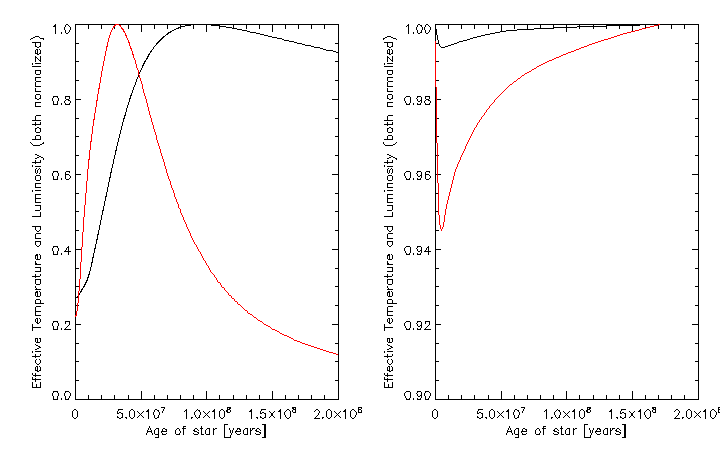
\includegraphics[width=6.0in]{fig3.png}
\caption{This plot shows how both temperature (black line) and luminosity (red 
line) change with a star's age. Model 1 is plotted on the left and Model 2 is 
plotted on the right.}
\label{fig3}
 \end{figure}



Stars remain stable against collapse because their internal outward pressure
balances the internal pressure due to gravity.
This internal pressure comes from several sources, such as electron
degeneracy, ideal gas, and radiation pressure from the photons produced
during nuclear reactions. A star with no nuclear reacations will thus have
a lower internal pressure. As it evolves, 
the star's temperature will
increase until the internal pressure can no longer balance the
pressure due to gravity. At this point, both temperature and luminosity
start to decrease as the star collapses, which happens at an age of around
 50 million years. This turnaround point is illustrated in 
the upper right hump in the lefthand plot in figure \ref{fig1}.




\end{document}


